\documentclass[../thesis.tex]{subfiles}
\begin{document}

\chapter{Preliminaries}
\label{ch:prelim}
\section{Data}
We use Quandl, a financial data platform, to obtain the different stock ticker data. Specifically, we used the WIKI and AS500 datasets to acquire stock data. The former contains end-of-day stock pricing data while the former contains intraday data, with updated pricing for each minute in the day. 

To acquire tweets from the companies, we use a slightly modified version of Github user \textit{bpb27}'s repository \textit{twitter\_scraping} \footnote{https://github.com/bpb27/twitter\_scraping}. Twitter doesn't make downloading all of the tweets easy or cost effective. Because we needed tweets from well over 10 years ago, and did not have the funding to use the Developer API's \texttt{get\_timeline()} method, we used this repository. This repository allows the user to circumvent Twitter's  3,200 tweet limit to pull potentially every single user's tweet. We used a powerful Colgate Computer Science Department server to perform hundreds of thousands of web requests; outputting the data into a CSV file for use in our implementation. We use 17 companies tweets and stock data for our experiments. 

\section{Stock Trading}
In this study we examine numerous algorithmic trading methods. To measure the effectiveness of a particular strategy, we use a quality metric to analyze productivity. Different denominations of purchasing powers are used and compared against a \textit {baseline measure}. The baseline measure is created by holding a long position of a specific denomination throughout the entire period of trading. Simply put, shares are bought at the beginning of the period and sold at the end. The profit level is then compared against the performance of the strategy. Much of the literature actively study the best performance of these strategies over different periods and use the same baseline comparison \cite{Liu2006}. We therefore include the same baseline in this study.

The stocks used in all strategies are found in Figure~\ref{stocktable}. These stocks were chosen given the availability of NASDAQ and S\&P500 stocks in the Quandl dataset and cover a variety of industries. This is important because we need to account for different performances of stocks. Certain large tech stocks like FB or GOOG have had incredible trajectories and performances whereas other stocks outside of the tech industry like HAS, have performed more moderately. The range of stocks chosen encompass nearly all of the major industries throughout the world.
\added[id=AT, remark = {update figure to include stocks used in twitter}] {Figure}

\textit {Buy} and \textit {sell signals} are thoroughly used throughout the study. Algorithms can generate a variety of buy and sell signals at a specific point in time, indicating that some denomination of stocks should be purchased or sold at that specific point in time. To measure how a given algorithm performs, different denominations of shares are purchased and compared. The strategies use closing price data from October 1st, 2006 to January 1st, 2017. Some strategies use intra-day stock data, which is minute-by-minute data of stock prices from October 26, 2018. Other additional terms need to be defined. \textit {Securities} and {\textit stocks } are used as terms interchangeably throughout the paper. Securities have more of a broad definition, as securities include stocks, bonds, mortgages, and others. \textit {Bearish signals} signal trends of downturn whereas \textit {bullish} signal positive, upward trends \cite{Aldridge2010}. 

Graphs can be interpreted as follows. Figure~\ref{SMAfigure} shows the Simple Moving Average strategy applied to GOOG. Purple triangles, which are angled upwards, are buy signals while black triangles angled downwards are sell signals. On June 2015, the strategy generated a sell signal, denoted by the black triangle. In the following couple of months, a subsequent buy signal was generated as denoted by the purple triangle. The orange line is the long moving average, the blue line is the short moving average, and the red line gives the price of GOOG throughout the time. 

\begin{figure}[h]
\centering
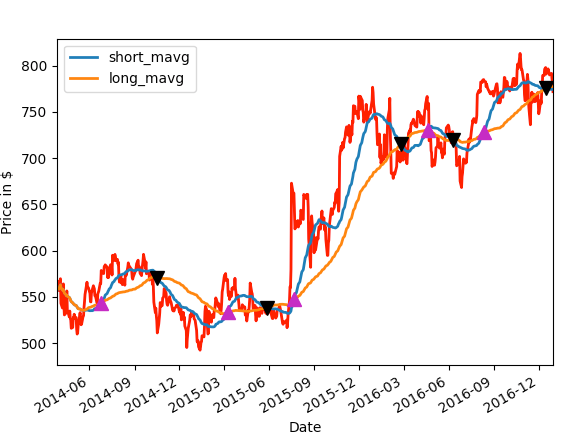
\includegraphics[width=90mm]{SMA_Google.png}
\caption{Simple Moving Average - "Golden Cross" Strategy applied to GOOG \label{overflow}}
\label{SMAfigure}
\end{figure}

\begin{figure}[h]
\centering
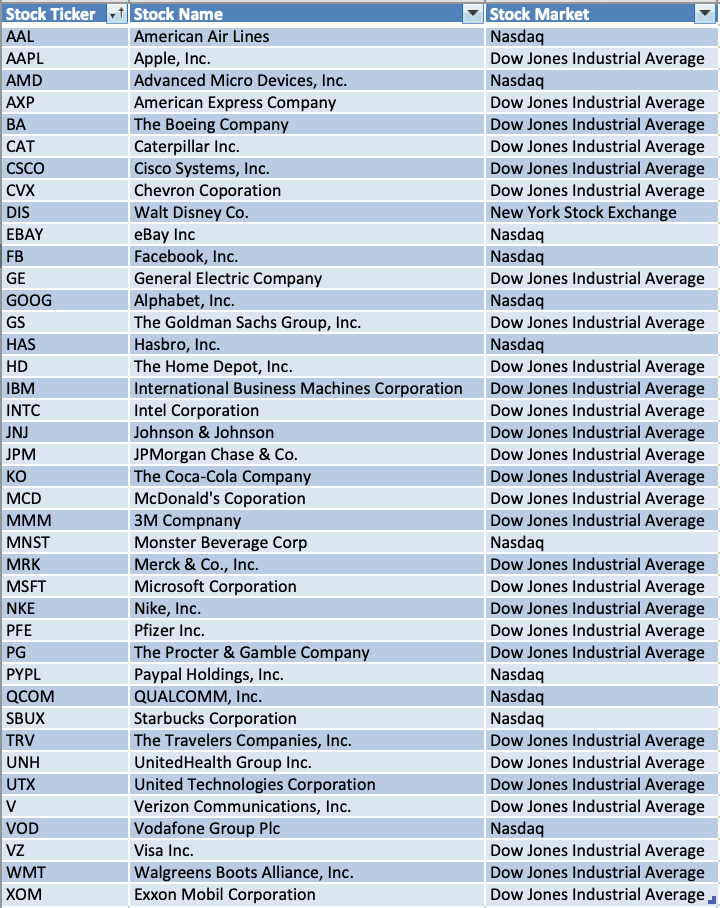
\includegraphics[width=85mm]{stock_table.png}
\caption{Table of stocks used in our study \label{overflow}}
\label{stocktable}
\end{figure}

\section{Stock Trading and Machine Learning Algorithms}
\added[id=AT, remark = {is this a necessary section to have?}] {do I need this section - yes 4 different discussions of ml/deep learning networks, TALK ABOUT WHAT EACH MODEL PREDICTS, 1 OR -1 OR PRICE}

Our implementation uses the both the Scikit-learn and TensorFlow Python libraries \cite{PedregosaFABIANPEDREGOSA2011} \cite{Abadi}. We use Natural Language Processing to conduct a sentiment analysis of tweets for our models. We then aggregate the twitter data across days of stock trading and then feed the combined stock and twitter data into a variety of different machine learning algorithms. 

\subsection{NLP}
Natural Language Processing (NLP) is a branch of artificial intelligence that allows machines to understand and decipher human language. For our implementation, we used the textblob python library to perform NLP on the Twitter data \cite{Loria2018}. We perform sentiment analysis on the text from the tweets and use the \textit{polarity} score, which is a float from -1 to 1, to understand the sentiment of individual tweets. The textblob library generates polarity from a na\"{i}ve Bayesian classifier that has been pre-trained on a movie review data corpus by identifying positive and negative words from the input text. 

\subsection{Decision Tree Classifier}
We use a decision tree classifier for one of our models from the Scikit-learn library. Decision trees are models that predict the value of a target variable by learning simple decision rules inferred from the data features \cite{PedregosaFABIANPEDREGOSA2011}. It breaks down a dataset into smaller and smaller subsets, with the leaf nodes  representing the classification prediction. Because we are using a classifier, our implementation predicts whether or not the following days closing price will be higher or lower, which is represented by a 1 or -1. Another benefit of decision trees is that they can be visualized easily. Figure~\ref{DecTreefigure} shows the decision tree fitted to DIS. However, due to the complexity of our model it is difficult to interpret the visualization. 

\begin{figure}[h]
\centering
\includegraphics[width=90mm]{decision_tree_DIS.pdf}
\caption{Decision Tree Visualization of DIS \label{overflow}}
\label{DecTreefigure}
\end{figure}

\subsection{RandomForest Regressor}
We use Scikit-learn's implementation of a RandomForest regressor. This module builds off of the above's section decision tree implementation. It instead uses a randomized decision tree making a diverse set of classifiers by introducing randomness in the classifier construction \cite{PedregosaFABIANPEDREGOSA2011}. This prediction of the ensemble is then given as an averaged prediction of the individual classifiers. Each tree in the ensemble when it is constructed is built from a random sample drawn from the training set. More randomness is added during construction by choosing the best split of nodes from a random subset of the features. This generally induces more bias from the randomness, but due to averaging often decreases variance and hence yields a better overall model \cite{PedregosaFABIANPEDREGOSA2011}. Unlike a classifier, a regressor is able to predict and model float values, giving us a different insight, as our implementation predicts the magnitude of change in closing price rather than just the direction of price movement. 

\subsection{MLP Classifier}
We use Scikit-learn's implementation of a multi-layer perceptron (MLP) classifier. MLPs are composed of multiple perceptrons, which are individual neural networks that perform binary classification. They have an input layer, a certain number of hidden layers, and an output layer which makes a decision about the given input and are generally used in a supervised learning context. The network \textit{learns} by using a back-propagation algorithm consisting of two steps \cite{Honkela2001}. In the forward pass, predicted outputs from a given input are evaluated mathematically. In the backwards pass, partial derivatives of the cost function are propagated back through the network. Figure~\ref{MLPgraph} shows how a signal flows through a simple MLP with one hidden layer. 

\begin{figure}[h]
\centering
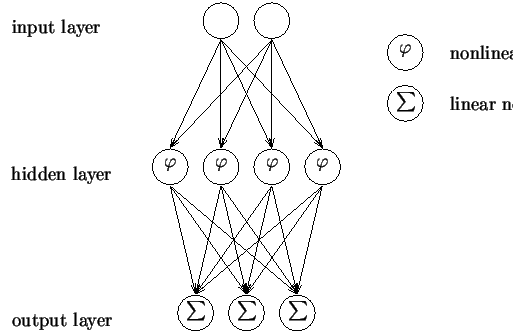
\includegraphics[width=90mm]{MLP_graph.png}
\caption{Signal-flow graph of an MLP \label{overflow}}
\label{MLPgraph}
\end{figure}

We choose a classifier with 3 hidden layers, each with 100 neurons, and use a stochastic gradient descent for the solver. While MLP classifiers can handle a variety of different layers and solvers, this combination proved to be most effective during testing of the algorithm for our combined Twitter and stock data. The MLP classifier predicts a 1 or -1, signaling a price rise or alternatively a price drop the following day. 

\subsection{$K$-nearest Neighbors Classifier}
We use Scikit-learn's implantation of the $k$- nearest neighbors classifier. This algorithm is one of the simplest machine learning algorithms that exists. After choosing a $k$, or amount of nearest neighbors, it calculates the distance between the query sample and all of the training samples via Euclidian distance \cite{PedregosaFABIANPEDREGOSA2011}. The algorithm then sorts the ordered collection of distances and chooses the mode of the $k$ selected labels for classification. In a regression, it would choose the mean of the $k$ selected labels. Because we are doing classification, our algorithm predicts binary price change, as in the other classification algorithms discussed above. 

\subsection{Deep Learning}
We implement an LSTM model using the TensorFlow Python library \cite{Abadi}. This is an example of a recurrent neural network (RNN). Unlike traditional neural networks, RNN's use previous data to help classify or predict the current value \cite{Colah2015}. RNN's have persistence and are networks with loops in them. Long Short Term Memory networks (LSTM) are a special type of RNN that is capable of learning long-term dependencies unliked traditional neural networks which struggle with this problem. They are trained via back-propogation over time and instead of neurons have memory blocks that are connected through layers. Each block contains 3 different types of gates which are triggered by sigmoid activation units: forget, input, and output gates. The first decides wether or not to throw away information from the block. The second decides which values from the input should be allocated to update the memory state. The third decides what to output based on input and memory state. Because the structure of an RNN allows the model to use past events to aid future states unlike a typical neural network, this has an ideal application for long term time-series based data, which makes an LSTM model ideal for our use case \cite{Colah2015}.

\added[id=AT, remark = {should i insert a graph?}] {should i give an explanation behind math/ graph??? - to be honest not entirely sure I understand it}

The model for our implementation has a look back of 60 days. At its core, our LSTM model processes 60 days prior of inputs including closing price, tweet sentiment, and a variety of Twitter data, and then predicts the following days closing price. Unlike the above methods which predict signaled change, this model predicts the stock price. Furthermore, we add a second layer into our model. This stacked LSTM makes the output of the first layer become the input to the second layer, giving our model more depth and accuracy. To verify that our model is accurately predicting the following days stock prices well, we check the efficacy of the predictions by looking at mean squared error regression loss. This is done in Scikit-learn metrics function call to \texttt{mean\_squared\_error()}. 





\end{document}
